\subsection{Operant Conditioning Chamber and Classical Conditioning}

There are multiple kinds of learning a successful AGI system can make use of; this environment focuses on Classical Conditioning using a na\"{i}ve Bayesian probability model.

An Operant conditioning chamber (also called a Skinner box) is an apparatus used in the study of animal behavior. %Jack, although these concepts are well-known in psychology, we still need to cite something here. Can you figure out what we need to cite?
Operant conditioning chambers contain at least one operandum (typically a lever) and a means of delivering a primary reinforcer (a reward/punishment pair, e.g. apple/poison). Some operant chambers incorporate lights, sounds and/or drawings to produce multiple stimuli and signify when food is available.

It is easy to construct an operant conditioning chamber in PAGI World. A dispenser is placed within grabbing distance of the agent which when grabbed can produce a primary reinforcer (apples or poison).  These objects have associated positive and negative `endorphins' which the agent can respond to just as an animal would. 


\begin{figure}[h]
\centering
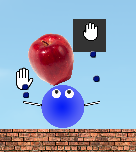
\includegraphics{dispenser}
\caption{PAGI World Operant Conditioning Chamber.} %expand on this caption a little---describe what we're looking at. Same applies to the next figure's caption.
\end{figure}


The application of such an environment is to test classical conditioning algorithms before full scale deployment.  One can limit the number of variables and focus solely on the agent's ability to interpret conditioned stimulus (CS)/unconditioned stimulus (US) pairs.

One such classical conditioning algorithm is implemented using a na\"{i}ve Bayesian probability model. %same here: please find out what a good citation is for this. Wikipedia itself isn't a good source, but it might point you to academic papers that are.
 The agent starts with the assumption that no action of his will lead to endorphins.  Once placed in the operant conditioning chamber, the agent tries to interact with the dispenser.  If this interaction with the dispenser produces endorphins, the CS-US pair is strengthened.  The strength of this CS-US pair is measured as a probability.

The agent is run through a number of tests, each time able to grab the dispenser a set number of times, or for a set period of time.  At the end of each trial, probabilities and the history of the dispenser are saved in a memory file to be used as the initial cases for the next trial.  PAGI World also has built in functions that allow one to change the dispenser's qualities.  This is used to replicate the phenomenon of extinction. %citation for extinction required. An introductory psychology textbook might suffice.


\begin{figure}[h]
\centering
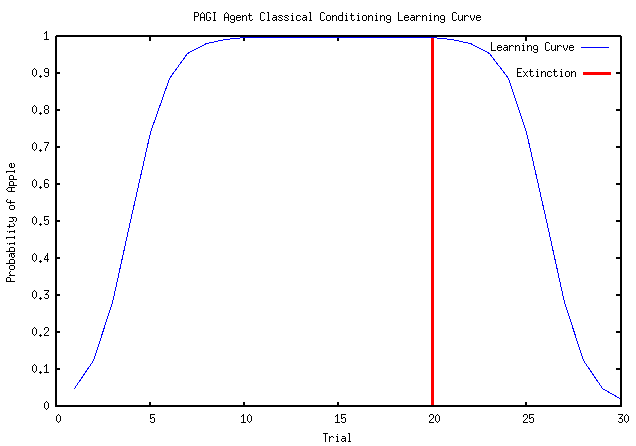
\includegraphics[scale=0.5]{cc_graph}
\caption{Agent Learning Curve}
\end{figure}

In this experiment the agent was provided with a dispenser that produced apples on every grab.  The graph shows the agent coming to this conclusion, as the probability of the dispenser dropping an apple rises to nearly one.  However, after 20 trials the dispenser is turned off.  The conditioned stimulus (grabbing the dispenser) is no longer paired with the conditioned response (endorphin increase due to apple).  Thus, a gradual weakening of the conditioned response can be observed, expressed on the graph as the decrease in the probability of an apple falling.  

This is just one simple example of the flexibility of PAGI World.  Both the operant conditioning chamber and example classical conditioning algorithm could be expanded to be more functional. %in what ways?